\documentclass[12pt]{exam}
\usepackage[utf8]{inputenc}
\usepackage{pdfpages}
\usepackage{amsmath,amstext,amsthm,amssymb,amsxtra, graphicx}
\usepackage[top=1.5in, bottom=1.5in, left=1.25in, right=1.25in]	{geometry}
%\usepackage[normalem]{ulem}
\usepackage{txfonts} % pxfonts txfonts 
\usepackage[T1]{fontenc}
\usepackage{lmodern}
\renewcommand*\familydefault{\sfdefault}
 \usepackage{euler}   % better than the option below
\usepackage{pdfsync}
\usepackage{multicol}
\newcommand{\ci}[1]{_{ {}_{\scriptstyle #1}}}
\graphicspath{ {images/} }


\newcommand{\norm}[1]{\ensuremath{\left\|#1\right\|}}
\newcommand{\abs}[1]{\ensuremath{\left\vert#1\right\vert}}
\newcommand{\ip}[2]{\ensuremath{\left\langle#1,#2\right\rangle}}
\newcommand{\p}{\ensuremath{\partial}}
\newcommand{\pr}{\mathcal{P}}

\newcommand{\pbar}{\ensuremath{\bar{\partial}}}
\newcommand{\db}{\overline\partial}
\newcommand{\D}{\mathbb{D}}
\newcommand{\B}{\mathbb{B}}
\newcommand{\Sp}{\mathbb{S}}
\newcommand{\T}{\mathbb{T}}
\newcommand{\R}{\mathbb{R}}
\newcommand{\Z}{\mathbb{Z}}
\newcommand{\C}{\mathbb{C}}
\newcommand{\N}{\mathbb{N}}
\newcommand{\Q}{\mathbb{Q}}
\newcommand{\mQ}{\mathcal{Q}}
\newcommand{\mS}{\mathcal{S}}
\newcommand{\scrH}{\mathcal{H}}
\newcommand{\scrL}{\mathcal{L}}
\newcommand{\td}{\widetilde\Delta}
\newcommand{\pw}{\text{PW}}
\newcommand{\esup}{\text{ess.sup}}
\newcommand{\Tn}{\mathcal{T}_n}
\newcommand{\Bn}{\mathbb{B}_n}
\newcommand{\rt}{\mathcal{O}}
\newcommand{\avg}[1]{\langle #1 \rangle}
\newcommand{\one}{\mathbbm{1}}
\newcommand{\eps}{\varepsilon}
\newcommand{\grad}{\nabla}

\newcommand{\La}{\langle }
\newcommand{\Ra}{\rangle }
\newcommand{\rk}{\operatorname{rk}}
\newcommand{\card}{\operatorname{card}}
\newcommand{\ran}{\operatorname{Ran}}
\newcommand{\osc}{\operatorname{OSC}}
\newcommand{\im}{\operatorname{Im}}
\newcommand{\re}{\operatorname{Re}}
\newcommand{\tr}{\operatorname{tr}}
\newcommand{\vf}{\varphi}
\newcommand{\f}[2]{\ensuremath{\frac{#1}{#2}}}

\newcommand{\kzp}{k_z^{(p,\alpha)}}
\newcommand{\klp}{k_{\lambda_i}^{(p,\alpha)}}
\newcommand{\TTp}{\mathcal{T}_p}
\newcommand{\m}[1]{\mathcal{#1}}
\newcommand{\md}{\mathcal{D}}
\newcommand{\qan}{\abs{Q}^{\alpha/n}}
\newcommand{\sbump}[2]{[[ #1,#2 ]]}
\newcommand{\mbump}[2]{\lceil #1,#2 \rceil}
\newcommand{\cbump}[2]{\lfloor #1,#2 \rfloor}

\newcommand{\hn}{{3}}
\newcommand{\dd}{{10-6}}
\newcommand{\class}{Aero 417}
\newcommand{\term}{Fall 2024}
\newcommand{\examnum}{Homework \hn: Due \dd}
\newcommand{\examdate}{}
\newcommand{\timelimit}{75 Minutes}
\newcommand{\vc}[3]{\langle #1,#2,#3\rangle}
\newcommand*{\vv}[1]{\vec{\mkern0mu#1}}
\newcommand{\bv}[1]{\boldsymbol{#1}}
\newcommand{\hide}[1]{}
\newcommand{\uvec}[1]{\boldsymbol{\hat{\textbf{#1}}}}
\newcommand{\vex}[1]{\boldsymbol{{\textbf{#1}}}}
\newcommand{\px}{\frac{\partial}{\partial x}}
\newcommand{\py}{\frac{\partial}{\partial y}}
\newcommand{\pt}{\frac{\partial}{\partial t}}
\newcommand{\pxx}{\frac{\partial^2}{\partial x^2}}
\newcommand{\pyy}{\frac{\partial^2}{\partial y^2}}
\newcommand{\ptt}{\frac{\partial^2}{\partial t^2}}


\pagestyle{head}
\firstpageheader{}{}{}
\runningheader{\class}{ Page \thepage\ of \numpages}{\examnum}
\runningheadrule

\makeatletter
\renewcommand*\env@matrix[1][*\c@MaxMatrixCols c]{%
  \hskip -\arraycolsep
  \let\@ifnextchar\new@ifnextchar
  \array{#1}}
\makeatother

\printanswers
\begin{document}

\noindent
\begin{tabular*}{\textwidth}{l @{\extracolsep{\fill}} r @{\extracolsep{6pt}} l}
\textbf{\class} & \textbf{Name:} & \makebox[2in]{\bf{Benjamin Tollison}}\\
\end{tabular*}\\
\rule[2ex]{\textwidth}{2pt}
%
\begin{questions}
\begin{question}
Why centrifugal compressors are not used in long-range aircraft as a component of the main
engines?
\end{question}
\begin{solutionorbox}[\stretch{1}]
Starting with the breguet's range equation:
\[S = \frac{L}{D} \eta_0 \frac{\text{LHV}}{g} \ln \left(\frac{m_0}{m_f}\right)\]
we will assume that the aircraft will have the same take-off weight and same dry weight and the 
only thing that we are changing is going to be the compressor geometry. Therefore the compressor
will only effect the overall efficency \(\eta_0\)
\begin{align*}
\begin{cases}
  V_\infty = 300  \frac{m}{s}\\
  V_e = 800  \frac{m}{s}\\
  P_e = 80  \text{kPa}\\
  P_{\text{atm}} = 20  \text{kPa} \\
  A_e = 4 \, m^2 \\
  \dot{m} = 10  \frac{kg}{s}
\end{cases}
\end{align*}

\[T = \dot{m} V_e - \dot{m} V_\infty + A_e (P_e - P_{\text{atm}})\]
\[\therefore T = 245 \text{kN}\]

\end{solutionorbox}

\newpage 
\begin{question}
Describe the differences between Brayton Cycle and a Real Gas Turbine Cycle. Make
diagrams to explain the losses associated with a real engine.
\end{question}
\begin{solutionorbox}[\stretch{1}]
\[\]
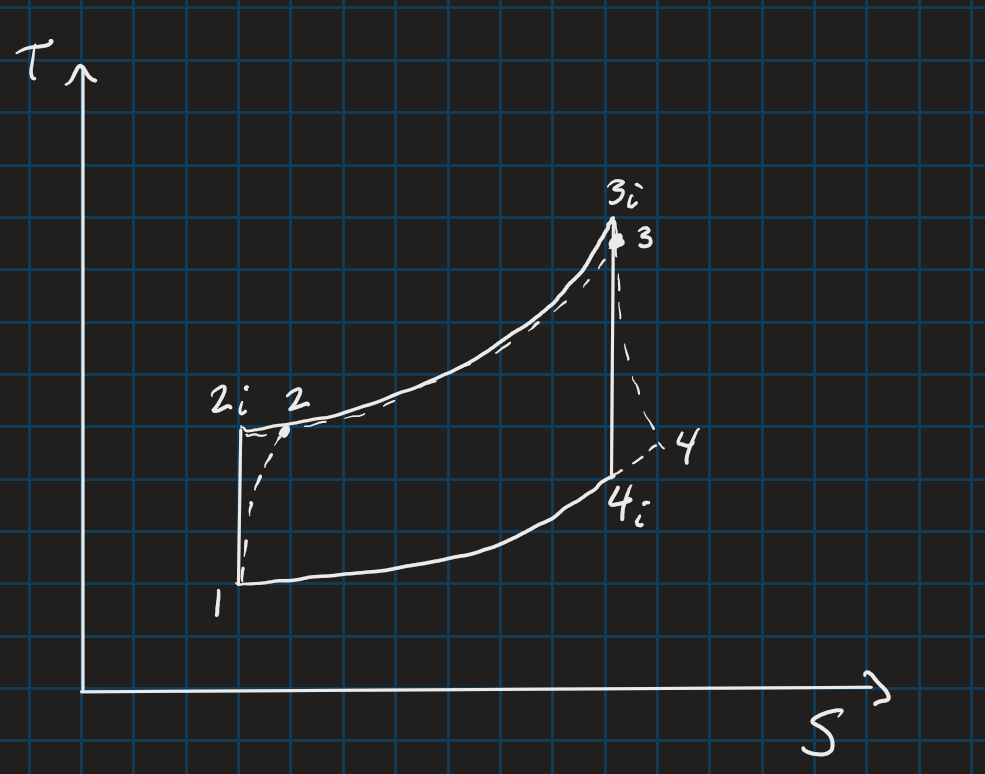
\includegraphics[width=\linewidth]{brayton v real cycle.png}
The first losses occur in the compressor from stage 1->2 due to the 
flow not being reversible. The combustion process is not completely isobaric.
The process in the turbine is also not reversible.
\end{solutionorbox}


\newpage 
\begin{question}
Draw the T-s diagram and determine the turbine shaft power, and the air-fuel ratio
\end{question}
\begin{solutionorbox}[\stretch{1}]
With all the given infomation the only equations used to find the shaft power were:
\[P_{02} = rP_{01}\]
\[T_{02} = T_{01}\left[1 + \frac{1}{\eta_c}\left(r^\frac{\gamma-1}{\gamma} - 1\right)\right]\]
\[W_* = \frac{1}{\eta_*}cp_*(T_i - T_j)\]
\[\text{P} = \dot{m}_{gas}(W_T - W_C)\]
\(\therefore \text{P}_{shaft} = 5740.3282\) [kW] 

The entropy starting values were pulled from Dr.Cizmas' textbook from the 
air tables for \(s_1\) and stoichiometric tables for \(s_3\). The following equation
was used to find the other two values:
\[s_i - s_j = cp_*\ln{\frac{T_i}{T_j}} - R\ln{\frac{P_i}{P_j}}\]
which then produces the following T-s graph.
\begin{center}
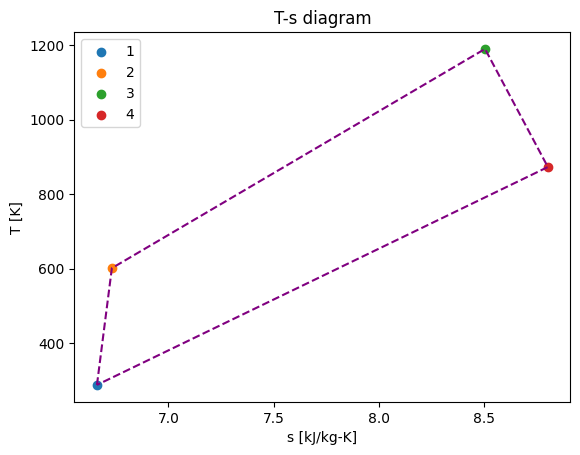
\includegraphics[width=350pt]{t-s-graph.png}
\end{center}
The ideal fuel to air ratio was pulled from the 5th set of lecture slides:
\[\Delta{t_c} = 588.4864 \rightarrow f \approx 0.014\]
\[\therefore f^{-1} \approx 71.429\]

\end{solutionorbox}

\end{questions}

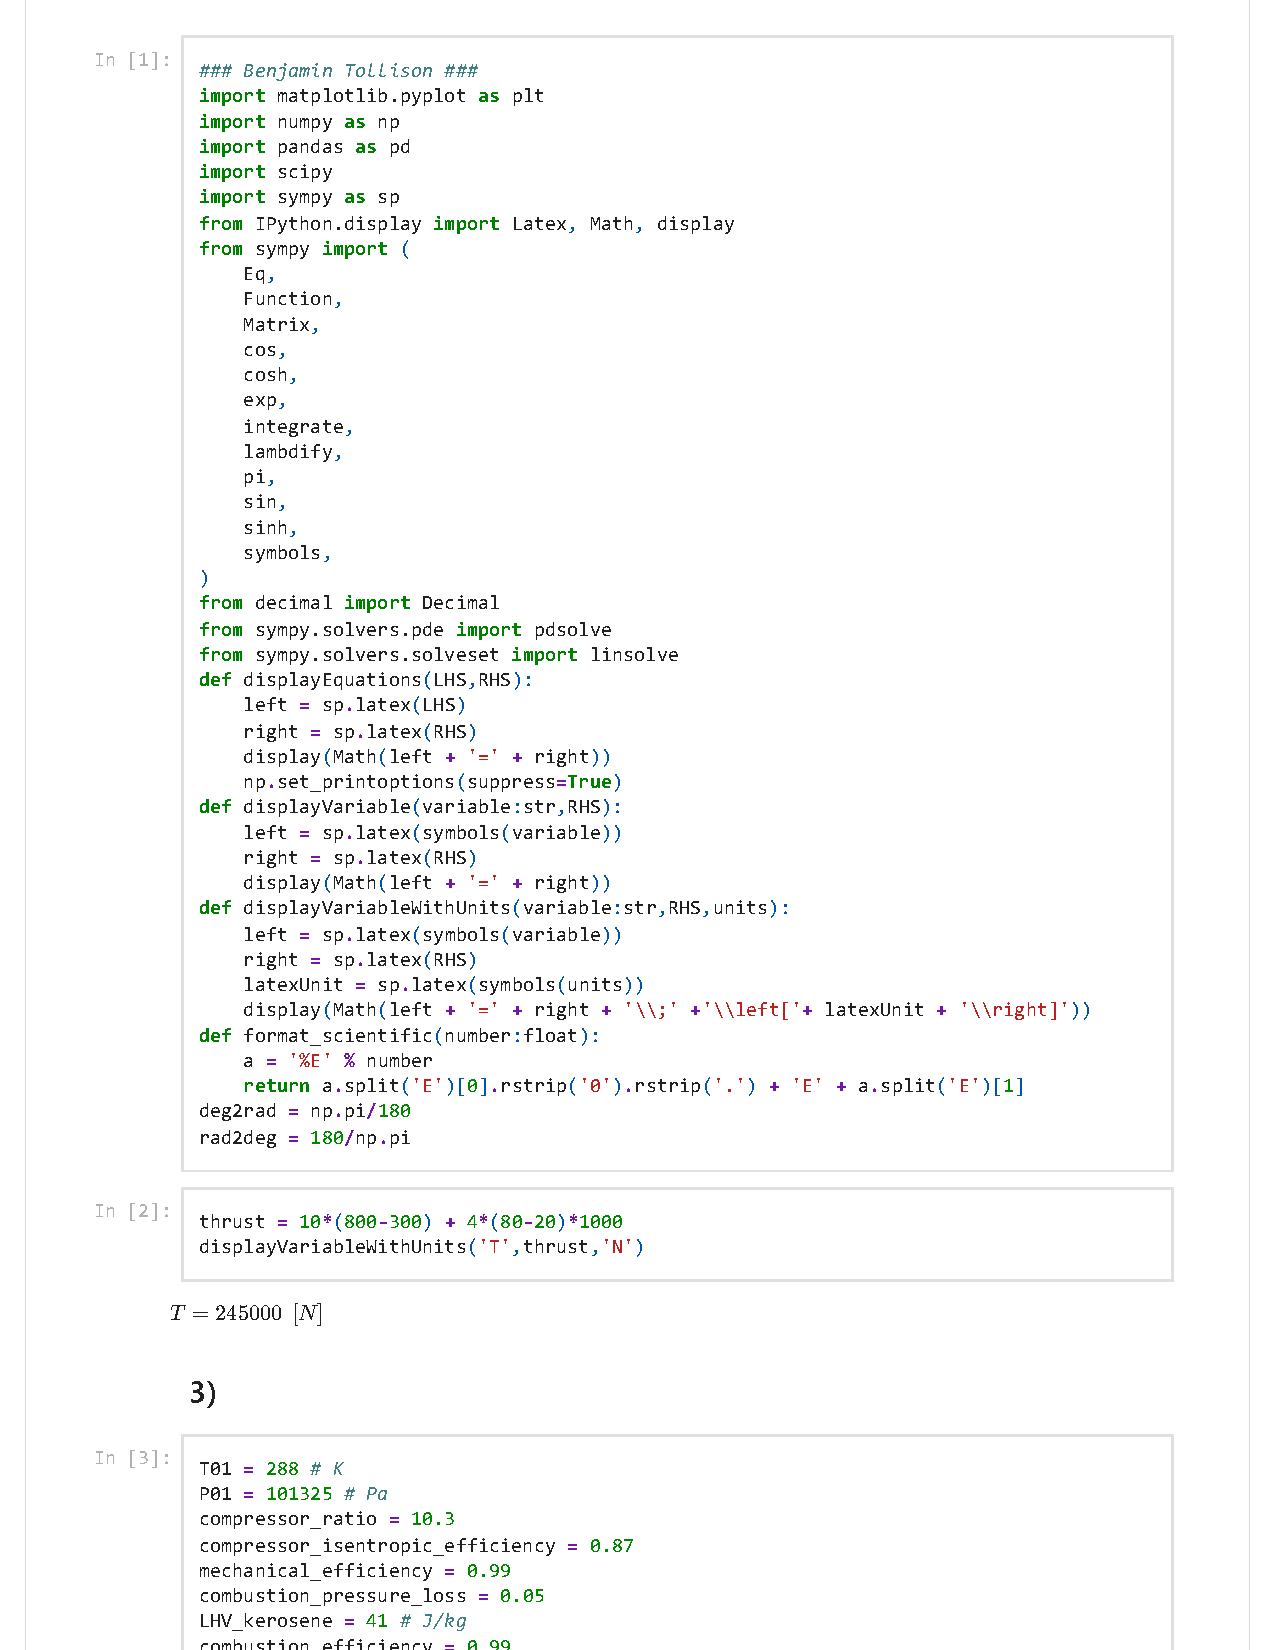
\includepdf[pages=-]{hw2-calculations.pdf}
\end{document}
